\documentclass[aspectratio=169]{beamer}
\usepackage{tikz}
\usepackage{xcolor}
\usetikzlibrary{shapes.geometric, arrows.meta, positioning, fit, backgrounds, shadows, decorations.pathreplacing, calc}

% Theme
\usetheme{Madrid}
\usecolortheme{beaver}

% Custom colors
\definecolor{frontend}{RGB}{70, 130, 180}      % Steel blue
\definecolor{execution}{RGB}{60, 179, 113}     % Medium sea green
\definecolor{detection}{RGB}{220, 20, 60}      % Crimson
\definecolor{verification}{RGB}{148, 0, 211}   % Dark violet
\definecolor{oracle}{RGB}{255, 140, 0}         % Dark orange
\definecolor{lightgray}{RGB}{240, 240, 240}    % Light background

\title{PythonFromScratch}
\subtitle{Static Analysis with Symbolic Execution \& Barrier Certificates}
\date{\today}

\begin{document}

% ============================================================================
% TITLE SLIDE
% ============================================================================
\begin{frame}[plain,noframenumbering]
\titlepage
\end{frame}

% ============================================================================
% SLIDE 1: System Architecture Overview
% ============================================================================
\begin{frame}{System Architecture Overview}
\centering
\vspace{-0.2cm}
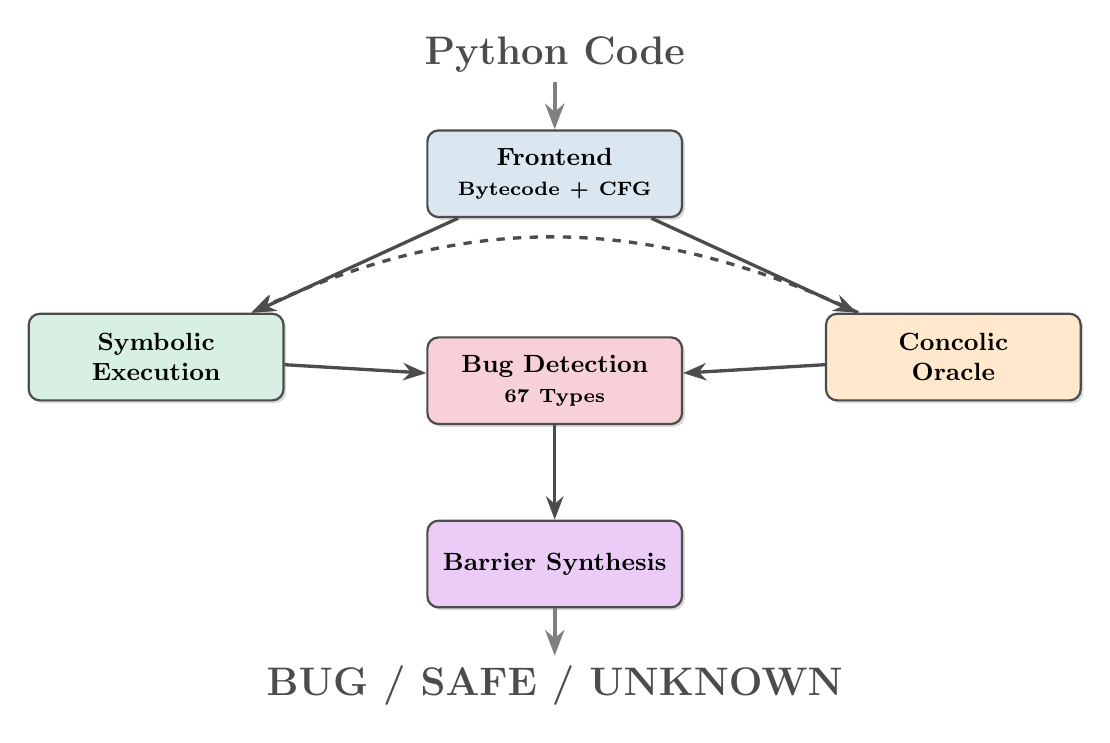
\begin{tikzpicture}[
    node distance=1.2cm and 1.8cm,
    component/.style={
        rectangle, rounded corners=4pt, 
        minimum width=3.2cm, minimum height=1.1cm,
        text width=3cm, align=center,
        draw=black!70, line width=0.8pt,
        font=\small\bfseries,
        drop shadow={opacity=0.3, shadow xshift=1pt, shadow yshift=-1pt}
    },
    arrow/.style={
        -Stealth, line width=1.2pt, draw=black!70
    }
]

% Main components
\node[component, fill=frontend!20] (frontend) at (0, 0) {Frontend\\{\scriptsize Bytecode + CFG}};
\node[component, fill=execution!20, below left=of frontend] (symbolic) {Symbolic\\Execution};
\node[component, fill=oracle!20, below right=of frontend] (concolic) {Concolic\\Oracle};
\node[component, fill=detection!20, below=1.5cm of frontend] (detection) {Bug Detection\\{\scriptsize 67 Types}};
\node[component, fill=verification!20, below=of detection] (verification) {Barrier Synthesis};

% Arrows
\draw[arrow] (frontend) -- (symbolic);
\draw[arrow] (frontend) -- (concolic);
\draw[arrow] (symbolic) -- (detection);
\draw[arrow] (concolic) -- (detection);
\draw[arrow] (detection) -- (verification);
\draw[arrow, dashed, bend right=25] (concolic) to (symbolic);

% Input/Output
\node[above=0.6cm of frontend, font=\Large\bfseries, color=black!70] (input) {Python Code};
\draw[arrow, color=black!50, line width=1.4pt] (input) -- (frontend);

\node[below=0.6cm of verification, font=\Large\bfseries, color=black!70] (output) {BUG / SAFE / UNKNOWN};
\draw[arrow, color=black!50, line width=1.4pt] (verification) -- (output);

\end{tikzpicture}

\vspace{0.3cm}
\begin{center}
\small
\textbf{Modes:} Intraprocedural • Interprocedural • Function Entry Points\\
\textbf{Backend:} Z3 SMT Solver • SOS/SDP Optimization
\end{center}
\end{frame}

% ============================================================================
% SLIDE 2: Symbolic Execution & Taint Tracking
% ============================================================================
\begin{frame}{Symbolic Execution \& Taint Tracking}
\vspace{-0.2cm}

\begin{columns}[T]
\column{0.48\textwidth}
\begin{block}{Symbolic Execution}
\small
\textbf{Path Exploration:}
\begin{itemize}\itemsep2pt
    \item Z3-based constraint solving
    \item Path-sensitive analysis
    \item Loop unrolling \& bounds
    \item Branch coverage tracking
\end{itemize}

\vspace{0.2cm}
\textbf{State Management:}
\begin{itemize}\itemsep2pt
    \item Symbolic heap modeling
    \item Variable tracking
    \item Context sensitivity (k-CFA)
\end{itemize}
\end{block}

\column{0.48\textwidth}
\begin{block}{Taint Analysis}
\small
\textbf{Taint Sources:}
\begin{itemize}\itemsep2pt
    \item User input (stdin, args)
    \item Network data (HTTP, sockets)
    \item File I/O, environment vars
    \item Function parameters (security mode)
\end{itemize}

\vspace{0.2cm}
\textbf{Propagation:}
\begin{itemize}\itemsep2pt
    \item Intra-procedural flow
    \item Inter-procedural with summaries
    \item Container operations
\end{itemize}
\end{block}
\end{columns}

\vspace{0.3cm}
\begin{center}
\footnotesize
\textbf{Concolic Oracle:} Concrete execution validates symbolic paths and refines constraints
\end{center}

\end{frame}

% ============================================================================
% SLIDE 2b: Symbolic vs Concolic Roles
% ============================================================================
\begin{frame}{Symbolic vs Concolic Execution: Complementary Roles}
\vspace{-0.5cm}

\begin{columns}[T]
\column{0.48\textwidth}
\begin{block}{Symbolic Execution}
\footnotesize
\textbf{Role:} Explore \textit{all possible} execution paths

\vspace{0.2cm}
\textbf{Strengths:}
\begin{itemize}\itemsep2pt
    \item Complete path coverage (in theory)
    \item Discovers edge cases automatically
    \item Generates constraints for all branches
    \item No need for test inputs
\end{itemize}

\vspace{0.2cm}
\textbf{Challenges:}
\begin{itemize}\itemsep2pt
    \item Path explosion in large programs
    \item Complex constraints (solver timeouts)
    \item Environmental interactions
\end{itemize}
\end{block}

\column{0.48\textwidth}
\begin{block}{Concolic Oracle}
\footnotesize
\textbf{Role:} \textit{Validate \& refine} symbolic reasoning

\vspace{0.2cm}
\textbf{Strengths:}
\begin{itemize}\itemsep2pt
    \item Grounds symbolic with concrete values
    \item Resolves constraint ambiguities
    \item Handles complex operations (hashing, crypto)
    \item Pruning infeasible paths
\end{itemize}

\vspace{0.2cm}
\textbf{Integration:}
\begin{itemize}\itemsep2pt
    \item Symbolic finds paths $\rightarrow$ Concolic validates
    \item Concolic provides counterexamples
    \item Hybrid: symbolic breadth + concrete depth
\end{itemize}
\end{block}
\end{columns}

\vspace{0.3cm}
\begin{center}
\scriptsize
\textbf{Best of Both:} Symbolic exploration + Concrete validation = Robust static analysis
\end{center}

\end{frame}

% ============================================================================
% SLIDE 3: Bug Detection Coverage
% ============================================================================
\begin{frame}{Bug Detection Coverage (67 Types)}
\vspace{-0.3cm}

\begin{columns}[T]
\column{0.48\textwidth}
\begin{block}{Security Vulnerabilities (47)}
\footnotesize
\textbf{Injection Attacks:}
\begin{itemize}\itemsep1pt
    \item SQL, Command, Code, Path
    \item LDAP, XPath, NoSQL, Regex
    \item Header, Cookie injection
\end{itemize}

\textbf{XSS \& Web:}
\begin{itemize}\itemsep1pt
    \item Reflected XSS, Stored XSS
    \item CSRF, Open Redirect
    \item Jinja2 autoescape issues
\end{itemize}

\textbf{Deserialization:}
\begin{itemize}\itemsep1pt
    \item Unsafe Pickle, YAML
    \item XXE, XML Bomb
\end{itemize}
\end{block}

\column{0.48\textwidth}
\begin{block}{\phantom{Security Vulnerabilities (47)}}
\footnotesize
\textbf{Crypto \& Data:}
\begin{itemize}\itemsep1pt
    \item Weak crypto (MD5, SHA1)
    \item Hardcoded credentials
    \item Cleartext logging/storage
    \item Insecure protocols (HTTP, FTP)
\end{itemize}

\textbf{Network \& Files:}
\begin{itemize}\itemsep1pt
    \item SSRF, Bind to 0.0.0.0
    \item Tar slip, Path traversal
    \item Weak file permissions
\end{itemize}

\textbf{Core Bugs (20):}
\begin{itemize}\itemsep1pt
    \item Bounds, Div-Zero, Null Ptr
    \item Type Errors, Overflows
    \item Non-Termination, Races
\end{itemize}
\end{block}
\end{columns}

\end{frame}

% ============================================================================
% SLIDE 4: Analysis Workflow
% ============================================================================
\begin{frame}{Analysis Workflow}
\centering
\vspace{-0.7cm}
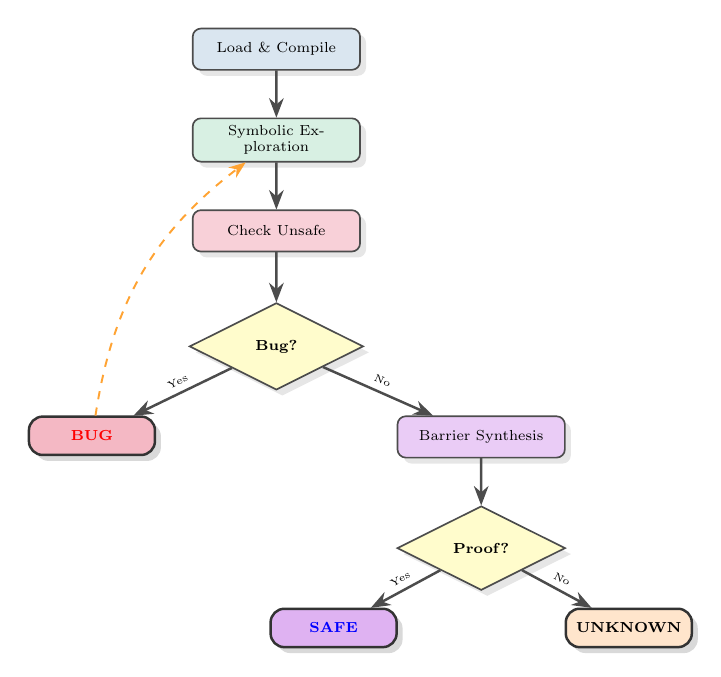
\begin{tikzpicture}[
    scale=0.75, transform shape,
    node distance=0.8cm and 1.5cm,
    process/.style={
        rectangle, rounded corners=3pt,
        minimum width=2.8cm, minimum height=0.7cm,
        text width=2.6cm, align=center,
        draw=black!70, line width=0.6pt,
        font=\scriptsize,
        drop shadow={opacity=0.2}
    },
    decision/.style={
        diamond, aspect=2,
        minimum width=2.2cm, minimum height=0.8cm,
        text width=1.8cm, align=center,
        draw=black!70, line width=0.6pt,
        font=\scriptsize\bfseries,
        drop shadow={opacity=0.2}
    },
    terminal/.style={
        rectangle, rounded corners=5pt,
        minimum width=2.1cm, minimum height=0.65cm,
        text width=1.9cm, align=center,
        draw=black!80, line width=0.9pt,
        font=\scriptsize\bfseries,
        drop shadow={opacity=0.3}
    },
    arrow/.style={
        -Stealth, line width=0.9pt, draw=black!70
    }
]

% Workflow
\node[process, fill=frontend!20] (load) at (0, 0) {Load \& Compile};
\node[process, fill=execution!20, below=of load] (explore) {Symbolic Exploration};
\node[process, fill=detection!20, below=of explore] (check) {Check Unsafe};

\node[decision, fill=yellow!20, below=0.85cm of check] (bugfound) {Bug?};

% Left path: BUG
\node[terminal, fill=detection!30, below left=0.8cm and 1.3cm of bugfound] (bug) {\textcolor{red}{BUG}};

% Right path: Try proof
\node[process, fill=verification!20, below right=0.8cm and 1.3cm of bugfound] (synthesize) {Barrier Synthesis};

\node[decision, fill=yellow!20, below=0.8cm of synthesize] (proofsuccess) {Proof?};

\node[terminal, fill=verification!30, below left=0.65cm and 0.7cm of proofsuccess] (safe) {\textcolor{blue}{SAFE}};
\node[terminal, fill=orange!20, below right=0.65cm and 0.7cm of proofsuccess] (unknown) {UNKNOWN};

% Main flow arrows
\draw[arrow] (load) -- (explore);
\draw[arrow] (explore) -- (check);
\draw[arrow] (check) -- (bugfound);
\draw[arrow] (bugfound) -- node[above, sloped, font=\tiny] {Yes} (bug);
\draw[arrow] (bugfound) -- node[above, sloped, font=\tiny] {No} (synthesize);
\draw[arrow] (synthesize) -- (proofsuccess);
\draw[arrow] (proofsuccess) -- node[above, sloped, font=\tiny] {Yes} (safe);
\draw[arrow] (proofsuccess) -- node[above, sloped, font=\tiny] {No} (unknown);

% Feedback loop
\draw[arrow, dashed, bend left=22, color=oracle!80, line width=0.7pt] (bug) to (explore);

\end{tikzpicture}

\vspace{0.2cm}
\begin{center}
\footnotesize
\textbf{Input:} Module • Functions • Interprocedural \quad
\textbf{Output:} Trace or Certificate
\end{center}
\end{frame}

% ============================================================================
% SLIDE 5: Barrier Synthesis Core Concept
% ============================================================================
\begin{frame}{Barrier Synthesis: Core Concept}
\vspace{-0.3cm}

\begin{block}{What is a Barrier Certificate?}
\small
A \textbf{barrier function} $B(x)$ separates the \textcolor{blue}{reachable states} from \textcolor{red}{unsafe states}:
\begin{itemize}\itemsep2pt
    \item $B(x) \geq 0$ for all initial states
    \item $B(x) < 0$ for all unsafe states
    \item $B(x)$ remains non-negative along all program executions (inductive)
\end{itemize}
If such $B$ exists, the program is provably \textbf{SAFE}.
\end{block}

\begin{columns}[T]
\column{0.48\textwidth}
\begin{block}{Synthesis Challenge}
\footnotesize
\textbf{Goal:} Find $B(x)$ automatically

\textbf{Approaches in 20 Papers:}
\begin{itemize}\itemsep1pt
    \item \textbf{Direct:} Polynomial templates + SOS/SDP
    \item \textbf{Abstraction:} Simplify state space, refine on failure
    \item \textbf{Learning:} Generate candidates from examples
    \item \textbf{Symbolic:} IC3/PDR, CHC solving
\end{itemize}
\end{block}

\column{0.48\textwidth}
\begin{block}{5-Layer Integration}
\footnotesize
\textbf{Layer 1-2:} Mathematical foundations + certificate types = \textit{core synthesis engine}

\textbf{Layer 3:} CEGAR $\rightarrow$ abstracts state space, feeds simplified problems to L1-2

\textbf{Layer 4:} Learning $\rightarrow$ generates barrier \textit{templates} for L1-2 to validate

\textbf{Layer 5:} IC3/CHC $\rightarrow$ symbolic reasoning provides alternative barrier representations
\end{block}
\end{columns}

\vspace{0.2cm}
\begin{center}
\scriptsize
All layers ultimately \textbf{synthesize or validate barrier functions} that prove safety
\end{center}

\end{frame}

% ============================================================================
% SLIDE 5b: Barrier Theory Visualization
% ============================================================================
\begin{frame}{Barrier Theory: Visual Explanation}
\centering
\vspace{-0.5cm}
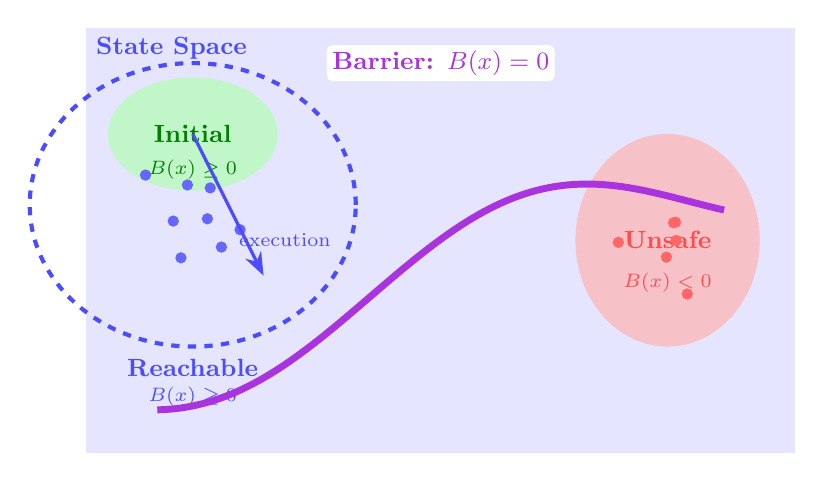
\begin{tikzpicture}[
    scale=0.9,
    state/.style={
        circle, draw, minimum size=0.15cm, inner sep=0pt
    }
]

% Draw regions
\fill[blue!10] (-5, -3) rectangle (5, 3);
\node[anchor=north west, font=\small\bfseries, blue!70] at (-5, 3) {State Space};

% Initial states region
\fill[green!30, opacity=0.7] (-3.5, 1.5) ellipse (1.2cm and 0.8cm);
\node[font=\small\bfseries, green!50!black] at (-3.5, 1.5) {Initial};
\node[font=\scriptsize, green!50!black] at (-3.5, 1) {$B(x) \geq 0$};

% Reachable states region (larger, encompasses initial)
\draw[blue!70, line width=1.5pt, dashed] (-3.5, 0.5) ellipse (2.3cm and 2cm);
\node[font=\small\bfseries, blue!70] at (-3.5, -1.8) {Reachable};
\node[font=\scriptsize, blue!70] at (-3.5, -2.2) {$B(x) \geq 0$};

% Unsafe states region
\fill[red!30, opacity=0.7] (3.2, 0) ellipse (1.3cm and 1.5cm);
\node[font=\small\bfseries, red!70] at (3.2, 0) {Unsafe};
\node[font=\scriptsize, red!70] at (3.2, -0.6) {$B(x) < 0$};

% Barrier function as a curve
\draw[verification!80, line width=2.5pt, domain=-4:4, samples=100] 
    plot (\x, {0.8*sin((\x+1)*40) + 0.3*\x - 0.5});
\node[font=\small\bfseries, verification!80, fill=white, rounded corners=2pt, inner sep=2pt] 
    at (0, 2.5) {Barrier: $B(x) = 0$};

% Add some sample state points
\foreach \i in {1,...,8} {
    \pgfmathsetmacro{\angle}{rand*360}
    \pgfmathsetmacro{\rad}{0.6 + rand*0.4}
    \pgfmathsetmacro{\x}{-3.5 + \rad*cos(\angle)}
    \pgfmathsetmacro{\y}{0.5 + 1.3*\rad*sin(\angle)}
    \fill[blue!60] (\x, \y) circle (0.08cm);
}

\foreach \i in {1,...,6} {
    \pgfmathsetmacro{\angle}{rand*360}
    \pgfmathsetmacro{\rad}{0.5 + rand*0.4}
    \pgfmathsetmacro{\x}{3.2 + \rad*cos(\angle)}
    \pgfmathsetmacro{\y}{\rad*sin(\angle)}
    \fill[red!60] (\x, \y) circle (0.08cm);
}

% Arrow showing direction
\draw[-Stealth, line width=1.2pt, blue!70] (-3.5, 1.5) -- (-2.5, -0.5);
\node[font=\scriptsize, blue!70] at (-2.2, 0) {execution};

\end{tikzpicture}

\vspace{0.2cm}
\begin{center}
\small
\textbf{Key Insight:} The barrier $B(x)$ acts as a \textit{mathematical fence}\\
\scriptsize
If no execution can cross from $B(x) \geq 0$ to $B(x) < 0$, the system is \textbf{safe}
\end{center}

\end{frame}

% ============================================================================
% SLIDE 6: Layer 1-3 Details
% ============================================================================
\begin{frame}{Barrier Synthesis \& Verification}
\vspace{-0.5cm}

\begin{block}{5-Layer SOTA Architecture}
\footnotesize
\textbf{Layer 1: Mathematical Foundations}
\begin{itemize}\itemsep1pt
    \item Positivstellensatz, Sum-of-Squares (SOS) \& SDP
    \item Lasserre hierarchy, Sparse SOS
\end{itemize}

\textbf{Layer 2: Certificate Types}
\begin{itemize}\itemsep1pt
    \item Hybrid barriers (discrete-continuous)
    \item Stochastic, exponential \& logarithmic barriers
\end{itemize}

\textbf{Layer 3: Abstraction \& Refinement}
\begin{itemize}\itemsep1pt
    \item CEGAR (Counter-Example Guided Refinement)
    \item Predicate abstraction with IMPACT
    \item Boolean program transformation
\end{itemize}
\end{block}

\end{frame}

\begin{frame}{Barrier Synthesis: Advanced Techniques}
\vspace{-0.3cm}

\begin{block}{Layers 4-5: Learning \& Verification}
\small
\textbf{Layer 4: Learning-Based Synthesis}
\begin{itemize}\itemsep2pt
    \item ICE (Implication, Counterexample, Equivalence) learning
    \item Houdini inference for inductive invariants
    \item SyGuS (Syntax-Guided Synthesis) for template instantiation
    \item Data-driven barrier candidate generation
\end{itemize}

\textbf{Layer 5: Advanced Verification}
\begin{itemize}\itemsep2pt
    \item IC3/PDR (Incremental Construction of Inductive Clauses)
    \item CHC (Constrained Horn Clauses) solving with Spacer
    \item DSOS/SDSOS (Diagonally dominant SOS) for scalability
    \item Assume-Guarantee compositional reasoning
\end{itemize}
\end{block}

\vspace{0.3cm}
\begin{center}
\footnotesize
\textbf{Feedback Loop:} L3 simplifies $\rightarrow$ L4 suggests templates $\rightarrow$ L1-2 validates $\rightarrow$ L5 provides fallback
\end{center}

\end{frame}

% ============================================================================
% FINAL SLIDE: Layer Feedback Diagram
% ============================================================================
\begin{frame}{Layer Feedback Architecture}
\centering
\vspace{-0.3cm}

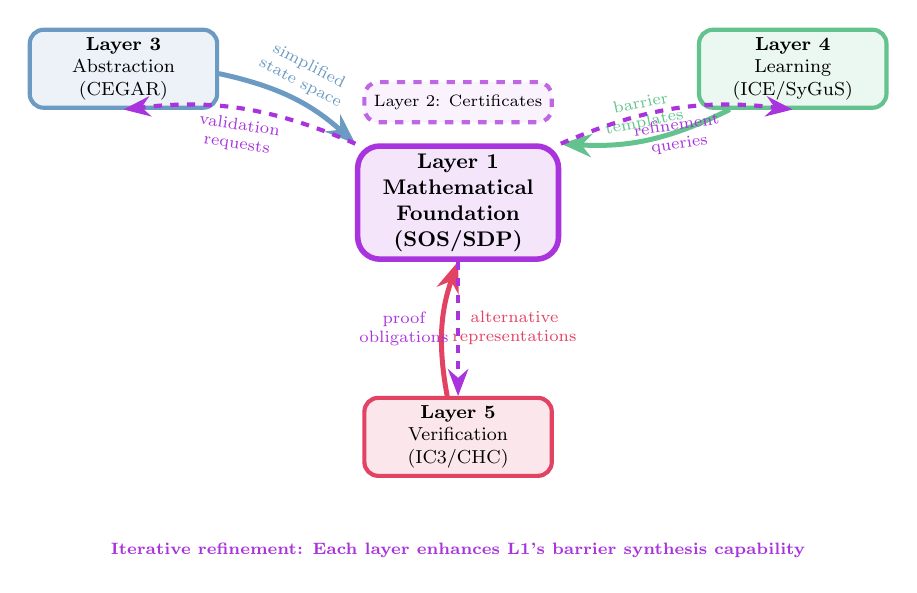
\begin{tikzpicture}[
    scale=0.85,
    transform shape,
    core/.style={rectangle, rounded corners=8pt, draw=verification!80, line width=2pt, 
                 fill=verification!10, minimum width=3cm, minimum height=1.5cm, align=center, font=\small\bfseries},
    layer/.style={rectangle, rounded corners=5pt, draw, line width=1.5pt, 
                  minimum width=2.8cm, minimum height=1cm, align=center, font=\footnotesize},
    feedback/.style={-Stealth, line width=1.8pt, bend left=15},
    label/.style={font=\scriptsize, align=center}
]

% Core Layer 1 (center)
\node[core] (L1) at (0, 0) {\textbf{Layer 1}\\Mathematical\\Foundation\\(SOS/SDP)};

% Layer 3 (left)
\node[layer, fill=frontend!10, draw=frontend!80] (L3) at (-5, 2) {\textbf{Layer 3}\\Abstraction\\(CEGAR)};

% Layer 4 (right)
\node[layer, fill=execution!10, draw=execution!80] (L4) at (5, 2) {\textbf{Layer 4}\\Learning\\(ICE/SyGuS)};

% Layer 5 (bottom)
\node[layer, fill=detection!10, draw=detection!80] (L5) at (0, -3.5) {\textbf{Layer 5}\\Verification\\(IC3/CHC)};

% Layer 2 (near L1)
\node[layer, fill=verification!5, draw=verification!60, dashed, minimum height=0.6cm, font=\scriptsize] (L2) at (0, 1.5) {Layer 2: Certificates};

% Feedback arrows from layers to L1
\draw[feedback, frontend!80] (L3) to node[label, above, sloped] {simplified\\state space} (L1.north west);
\draw[feedback, execution!80] (L4) to node[label, above, sloped] {barrier\\templates} (L1.north east);
\draw[feedback, detection!80] (L5) to node[label, right] {alternative\\representations} (L1.south);

% L1 outputs to higher layers
\draw[-Stealth, line width=1.5pt, verification!80, dashed] (L1.north west) to[bend right=15] 
      node[label, below, sloped] {validation\\requests} (L3.south);
\draw[-Stealth, line width=1.5pt, verification!80, dashed] (L1.north east) to[bend left=15] 
      node[label, below, sloped] {refinement\\queries} (L4.south);
\draw[-Stealth, line width=1.5pt, verification!80, dashed] (L1.south) to[bend left=0] 
      node[label, left] {proof\\obligations} (L5.north);

% Central loop annotation
\node[font=\scriptsize\bfseries, verification!80, fill=white, rounded corners=3pt, inner sep=3pt] at (0, -5.2) 
      {Iterative refinement: Each layer enhances L1's barrier synthesis capability};

\end{tikzpicture}

\end{frame}

\end{document}
